%!TEX program = xelatex
\documentclass[aspectratio=43,UTF8,10pt]{ctexbeamer}

    \mode<presentation> {
    \usetheme{Madrid}
    %\setbeamertemplate{footline} % To remove the footer line in all slides uncomment this line
    \setbeamertemplate{footline}[frame number] % To replace the footer line in all slides with a simple slide count uncomment this line
    \setbeamercolor{page number in head/foot}{fg=blue}
    \setbeamertemplate{navigation symbols}{} % To remove the navigation symbols from the bottom of all slides uncomment this line
    }
    \usepackage{indentfirst}
    \setlength{\parindent}{2em}
    \usepackage{listings}
    \lstset{language=C++, showstringspaces=false, basicstyle=\small}

    \usepackage{wrapfig}
    \usepackage{graphicx}
    % \usepackage{fboxrule}

    \definecolor{indiagreen}{rgb}{0.07, 0.53, 0.03}
    \definecolor{indianred}{rgb}{0.8, 0.36, 0.36}
    \definecolor{indianyellow}{rgb}{0.89, 0.66, 0.34}
    \definecolor{bondiblue}{rgb}{0.0, 0.58, 0.71}
    \definecolor{ao(english)}{rgb}{0.0, 0.5, 0.0}
    \definecolor{azure(colorwheel)}{rgb}{0.0, 0.5, 1.0}
    \definecolor{alizarin}{rgb}{0.82, 0.1, 0.26}
    % User Defined Block %%%%%%%%%%%%%%%%%%%%%%%%%%%%%%%%%%%%%%%%%%%%%%%%%%%%%%%%
    \newenvironment<>{abstractblock}[1]{%
      \setbeamercolor{block title}{fg=white,bg=bondiblue}%
    %   \setbeamercolor{block body}{fg=white,bg=bondiblue}%
      \begin{block}#2{#1}}{\end{block}}

    \newenvironment<>{adviceblock}[1]{%
    % \setbeamercolor{block title}{fg=white,bg=bondiblue}%
      \setbeamercolor{block body}{fg=white,bg=alizarin}%
    \begin{block}#2{#1}}{\end{block}}

    \newenvironment<>{thinkblock}[1]{%
      \setbeamercolor{block title}{fg=white,bg=azure(colorwheel)}%
    %   \setbeamercolor{block body}{fg=white,bg=bondiblue}%
      \begin{block}#2{#1}}{\end{block}}

    \newenvironment<>{yellowblock}[1]{%
      \setbeamercolor{block title}{fg=white,bg=indianyellow}%
      \begin{block}#2{#1}}{\end{block}}

    \lstset{language=C++,
    columns=flexible,
    basicstyle=\footnotesize\ttfamily,                                    % 设定代码字体、大小
    %numbers=left,xleftmargin=2em,framexleftmargin=2em,                   % 在左侧显示行号
    %numberstyle=\color{darkgray},                                        % 设定行号格式
    keywordstyle=\color{blue},                                            % 设定关键字格式
    commentstyle=\color{ao(english)},                                     % 设置代码注释的格式
    stringstyle=\color{brown},                                            % 设置字符串格式
    showstringspaces=false,                                              % 控制是否显示空格
    %frame=single,                                                         % 控制外框
    breaklines,                                                           % 控制是否折行
    % postbreak=\space,                                                     % 控制折行后显示的标识字符
    breakindent=5pt,                                                      % 控制折行后缩进数量
    emph={size\_t,array,deque,list,map,queue,set,stack,vector,string,pair,tuple,ostream}, % 非内置类型
    emphstyle={\color{teal}},
    escapeinside={(*@}{@*)},
}


    \title
        [第9章~继承与多态\hspace{2em}]
        {第9章~继承与多态}

    % \author
    %     []
    %     {}

    \date {}


    % \institute
    %     {}


\begin{document}

\maketitle





\begin{frame}
    {目录}
    \tableofcontents
\end{frame}

\begin{frame} {~~}
    \begin{yellowblock}{学习目标}
        \begin{itemize}
            \item 理解继承的内涵和基本语法;
            \item 掌握拷贝控制成员与继承的关系;
            \item 掌握并学会运用动态绑定技术。
        \end{itemize}
    \end{yellowblock}
\end{frame}

\section{继承}

\begin{frame}
    {9.1 继承\small{—定义基类和派生类}}
    \begin{exampleblock}{例9.1:}
        下面设计一个简单的人员系统,包括两类人员:学生(指大学生)和兼职员工。该系统包含以下几个类:Person、Student、PartTimeWorker和Course。\\
        ~~
    \end{exampleblock}

    \begin{figure}
    \centering
    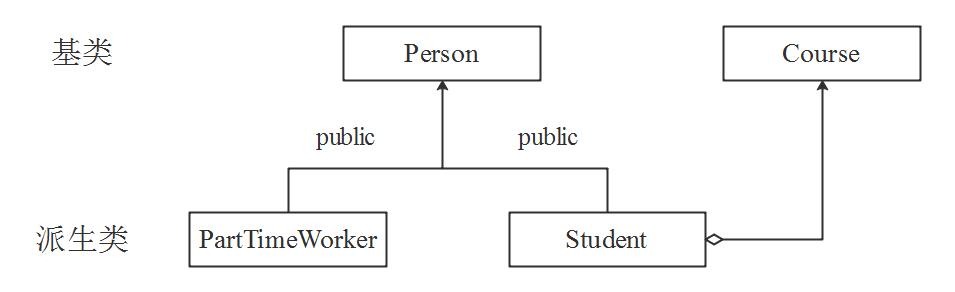
\includegraphics[width=25em]{Fig/Fig9-1.png}
    \end{figure}
\end{frame}
\subsection{定义基类}

\begin{frame}[fragile]
    {9.1 继承\small{—定义基类和派生类}}
    \begin{exampleblock}{例9.1中定义基类Person:}
    \begin{columns}
    \begin{column}{0.06\linewidth}
    \end{column}
    \begin{column}{0.94\linewidth}
    \begin{lstlisting}[]
class Person {                          //人员类
protected:
    string m_name;                      //名字
    int m_age;                          //年龄
public:
    Person(const string &name = "", int age = 0):m_name(name), m_age(age){}
    virtual ~Person() = default;        //default关键字见教材6.2.1节
    const string& name() const { return m_name; }
    int age() const { return m_age; }
    void plusOneYear() { ++m_age; }     //年龄自增
};
    \end{lstlisting}\ttfamily
    \end{column}
    \end{columns}
    \end{exampleblock}
\end{frame}

\begin{frame}[fragile]
    {9.1 继承\small{—定义基类和派生类}}
    \begin{exampleblock}{例9.1中定义基类Course:}
    \begin{columns}
    \begin{column}{0.06\linewidth}
    \end{column}
    \begin{column}{0.94\linewidth}
    \begin{lstlisting}[]
class Course {                 //课程类
    string m_name;             //课程名
    int m_score;               //成绩
public:
    Course(const string &name = "", int score = 0):
    m_name(name), m_score(score) {}
    void setScore(int score) { m_score = score; }
    int score() const { return m_score; }
    const string& name() const { return m_name; }
};
    \end{lstlisting}\ttfamily
    \end{column}
    \end{columns}
    \end{exampleblock}
\end{frame}
\subsection{定义派生类}

\begin{frame}[fragile]
    {9.1 继承\small{—定义基类和派生类}}
    \begin{exampleblock}{例9.1中定义派生类PartTimeWorker:}
    \begin{columns}
    \begin{column}{0.06\linewidth}
    \end{column}
    \begin{column}{0.94\linewidth}
    \begin{lstlisting}[]
class PartTimeWorker : public Person {  //兼职人员类,公有                                                        继承Person
private:
    double m_hour;                      //工作小时数
    static double ms_payRate;           //每小时工资
public:
    PartTimeWorker(const string &name, int age, double h=0):
    Person(name, age), m_hour(h){}
    void setHours(double h) { m_hour = h; }
    double salary() { return m_hour * ms_payRate; }
};
double PartTimeWorker::ms_payRate = 7.53;  //静态成员初始化
    \end{lstlisting}\ttfamily
    \end{column}
    \end{columns}
    \end{exampleblock}
\end{frame}

\begin{frame}[fragile]
    {9.1 继承\small{—定义基类和派生类}}
    \begin{exampleblock}{例9.1中定义派生类Student:}
    \begin{columns}
    \begin{column}{0.06\linewidth}
    \end{column}
    \begin{column}{0.94\linewidth}
    \begin{lstlisting}[]
class Student : public Person {  //学生类,公有继承Person
private:
    Course m_course;                 //课程信息
public:
    Student(const string &name, int age, const Course &c):
    Person(name, age), m_course(c) {}
    Course& course() { return m_course; }
};
    \end{lstlisting}\ttfamily
    \end{column}
    \end{columns}
    \end{exampleblock}
\end{frame}

\begin{frame}[fragile]
    {9.1 继承\small{—定义基类和派生类}}
    \begin{yellowblock}{提示:使用关键字\texttt{final}防止被继承}
    可以利用C++11提供的关键字final来阻止继承的发生:\\[0.5em]
    ~~ class NoDerived final \{\}; ~~~~  //NoDerived不能作为基类被继承
    \end{yellowblock}\vspace{2em}

    \begin{columns}
    \begin{column}{0.1\textwidth}
    \begin{beamercolorbox}[rounded=true, shadow=false,wd=0pt]{bgcolor}
    
\includegraphics[scale=0.6]{Fig/question_fig.jpg}
    \end{beamercolorbox}
    \end{column}

    \begin{column}{0.9\textwidth}
    \setbeamercolor{bgcolor}{fg=black,bg=green!50!white}
    \begin{beamercolorbox}[rounded=true, shadow=false,wd=10cm]{bgcolor}
    如果我们想让例9.1中派生类Student和PartTimeWorker不再被任何类继承,我们应该如何做?
    \end{beamercolorbox}
     \end{column}
    \end{columns}
\end{frame}

\subsection{访问控制}

\begin{frame}
    {9.1 继承\small{—访问控制}}
    \begin{block}{三类访问限定声明}
    a.该类中的函数~~b.派生类中的函数~~c.其友元函数~~d.该类的对象\vspace{0.5em}
    \begin{itemize}
    \item \textcolor[rgb]{0,0,1}{\texttt{public}} :可以被a、b、c和d访问。
    \item \textcolor[rgb]{0,0,1}{\texttt{protected}} :可以被a、b和c访问。
    \item \textcolor[rgb]{0,0,1}{\texttt{private}}:可以被a和c访问。
    \end{itemize}
    \end{block}
\end{frame}

\begin{frame}[fragile]
    {9.1 继承\small{—访问控制}}
    \begin{block}{下面代码正确吗?}
    \begin{columns}
    \begin{column}{0.06\linewidth}
    \end{column}
    \begin{column}{0.94\linewidth}
    \begin{lstlisting}[]
class Base {
private:
    int m_pri;          //private成员
protected:
    int m_pro;          //protected成员
public:
    int m_pub;          //public成员
};
class PubDerv : public Base {
    void foo() {
        m_pri = 10;     //错误:不能访问Base类私有成员
        m_pro = 1;      //正确:可以访问Base类受保护成员
    }
};
void test() {
    Base b;
    b.m_pro = 10; }       //错误:不能访问Base类受保护成员
    \end{lstlisting}\ttfamily
    \end{column}
    \end{columns}
    \end{block}
\end{frame}

\begin{frame}
    {9.1 继承\small{—访问控制}}
    \begin{block}{三类继承方式}
    \begin{itemize}
    \item \textcolor[rgb]{0,0,1}{\texttt{public}}~继承 :基类的protected和public属性在其派生类中\alert{保持不变}。
    \item \textcolor[rgb]{0,0,1}{\texttt{protected}}~继承 :基类的protected和public属性在派生类中变为protected。
    \item \textcolor[rgb]{0,0,1}{\texttt{private}}~继承:基类的protected和public属性在派生类中变为private。
    \end{itemize}
    以上三种继承,基类中的private属性在其派生类中均\alert{保持不变}。
    \end{block}\vspace{2em}
    \begin{yellowblock}{提示:公有继承是主流}
    由于私有继承和受保护继承均具有\alert{局限性},所以公有继承是主流的继承方式。
    \end{yellowblock}
\end{frame}

\begin{frame}[fragile]
    {9.1 继承\small{—访问控制}}
    \begin{block}{下面代码正确吗?}
    \begin{columns}
    \begin{column}{0.06\linewidth}
    \end{column}
    \begin{column}{0.94\linewidth}
    \begin{lstlisting}[]
class PriDerv : private Base {  //私有继承不影响派生类成员对                                              基类的访问
    void foo() {
        m_pro = 1;      //正确:可以访问Base类受保护成员
        m_pub = 1;      //正确:可以访问Base类公有成员
    }
};
void test() {
    PubDerv d1;
    PriDerv d2;
    d1.m_pub = 10;       //正确:m_pub在PubDerv中是公有的
    d2.m_pub = 1;        //错误:m_pub在PubDerv中是私有的
}
    \end{lstlisting}\ttfamily
    \end{column}
    \end{columns}
    \end{block}
\end{frame}

\begin{frame}[fragile]
    {9.1 继承\small{—访问控制}}
    \begin{block}{使用using声明}
        通过使用using声明,可以\alert{改变}派生类中基类成员的访问权限:
    \begin{columns}
    \begin{column}{0.06\linewidth}
    \end{column}
    \begin{column}{0.94\linewidth}
    \begin{lstlisting}[]
class PubDerv : public Base {
public:
    using base::m_pro;          //声明为公有的
};
void test() {
    PubDerv d;
    d.m_pro;                    //正确
}
    \end{lstlisting}\ttfamily
    \end{column}
    \end{columns}
    \end{block}
    \begin{alertblock}{注意:}
    派生类只能为它可以访问的名字提供using声明。
    \end{alertblock}
\end{frame}

\begin{frame}[fragile]
    {9.1 继承\small{—访问控制}}
    \begin{block}{命名冲突}
        如果派生类成员的名字和基类的成员名字相同,那么定义在派生类(内层作用域)的名字将会\alert{屏蔽}掉基类(外层作用域)的名字:
    \begin{columns}
    \begin{column}{0.06\linewidth}
    \end{column}
    \begin{column}{0.94\linewidth}
    \begin{lstlisting}[]
class Base {
protected:
    int m_data;
public:
    void foo(int) { /*...*/ }
};
class Derived : public Base {
protected:
    int m_data;                         //基类m_data被隐藏
public:
    int foo() {                         //基类foo成员被隐藏
        return m_data;                  //返回Derived::m_data
    }
};
    \end{lstlisting}\ttfamily
    \end{column}
    \end{columns}
    \end{block}
\end{frame}

\begin{frame}[fragile]
    {9.1 继承\small{—访问控制}}
    \begin{block}{命名冲突}
        如果在派生类里面需要访问基类的同名成员,则可以使用基类的作用域运算符:
    \begin{columns}
    \begin{column}{0.06\linewidth}
    \end{column}
    \begin{column}{0.94\linewidth}
    \begin{lstlisting}[]
class Derived : public Base {
    /*...*/
    int foo() { return Base::m_data; }       //返回Base中的m_data
};
    \end{lstlisting}\ttfamily
    \end{column}
    \end{columns}
    \end{block}
    \vspace{2em}
    \begin{columns}
    \begin{column}{0.1\textwidth}
    \begin{beamercolorbox}[rounded=true, shadow=false,wd=0pt]{bgcolor}
    
\includegraphics[scale=0.6]{Fig/question_fig.jpg}
    \end{beamercolorbox}
    \end{column}
    \begin{column}{0.9\textwidth}
    \setbeamercolor{bgcolor}{fg=black,bg=green!50!white}
    \begin{beamercolorbox}[rounded=true, shadow=false,wd=10cm]{bgcolor}
    如果我们想调用基类中的foo函数,我们应该如何做?
    \end{beamercolorbox}
    \end{column}
    \end{columns}
\end{frame}

\subsection{类型转换}

\begin{frame}[fragile]
    {9.1 继承\small{—类型转换}}
    \begin{block}{派生类到基类的转换}
         一个派生类不仅包含自己定义的(非静态)成员,而且还包含其从基类继承的成员。因此,可以将派生类对象当成基类对象使用,也就是说可以将基类的\alert{指针}或\alert{引用}与派生类对象\alert{绑定},例如:
    \begin{columns}
    \begin{column}{0.06\linewidth}
    \end{column}
    \begin{column}{0.94\linewidth}
    \begin{lstlisting}[]
PartTimeWorker w("Kevin", 21);
Person p, *ptr;
ptr = &w;                        //基类指针ptr指向派生类对象w
Person &p2 = w;                  //基类引用绑定到派生类对象w
p = w;                           //派生类对象赋值给基类对象
    \end{lstlisting}\ttfamily
    \end{column}
    \end{columns}
    \end{block}
\end{frame}

\begin{frame}[fragile]
    {9.1 继承\small{—类型转换}}
    \begin{block}{派生类到基类的转换}
         虽然派生类可以自动转换为基类的引用或指针,但没有从基类到派生类的自动转换。这是显而易见的,因为基类对象不能提供派生类对象\alert{新定义的部分},例如:
    \begin{columns}
    \begin{column}{0.06\linewidth}
    \end{column}
    \begin{column}{0.94\linewidth}
    \begin{lstlisting}[]
PartTimeWorker *w2 = &p;             //错误:不能将基类转换为派生类
w = p;                               //错误:不能将基类转换为派生类
    \end{lstlisting}\ttfamily
    \end{column}
    \end{columns}
        用派生类对象来创建一个基类对象:
    \begin{columns}
    \begin{column}{0.06\linewidth}
    \end{column}
    \begin{column}{0.94\linewidth}
    \begin{lstlisting}[]
PartTimeWorker w("Kevin", 21);       //派生类对象
Person p(w);                         //利用派生类对象构造基类对象
    \end{lstlisting}\ttfamily
    \end{column}
    \end{columns}
        如果派生类以私有方式或受保护的方式继承基类,那么派生类将\alert{不能自动转换}为基类类型,例如:
    \begin{columns}
    \begin{column}{0.06\linewidth}
    \end{column}
    \begin{column}{0.94\linewidth}
    \begin{lstlisting}[]
PriDerv d;                           //priDerv私有继承Base
Base b(d);                           //错误:PriDerv不能转换为Base
    \end{lstlisting}\ttfamily
    \end{column}
    \end{columns}
    \end{block}
\end{frame}

\begin{frame}
    {9.1 继承\small{—类型转换}}
    \begin{yellowblock}{提示:从派生类到基类的转换原则}
        理解从派生类到基类的\alert{隐式自动转换}需要明白三点:
    \begin{itemize}
    \item 这种转换只限于指针或引用类型;
    \item 转换的前提是公有继承;
    \item 没有从基类到派生类的隐式自动转换。
    \end{itemize}
    \end{yellowblock}
\end{frame}

\section{构造、拷贝控制与继承}

\begin{frame}[fragile]
    {9.2 构造、拷贝控制与继承}
\begin{figure}
  \centering
  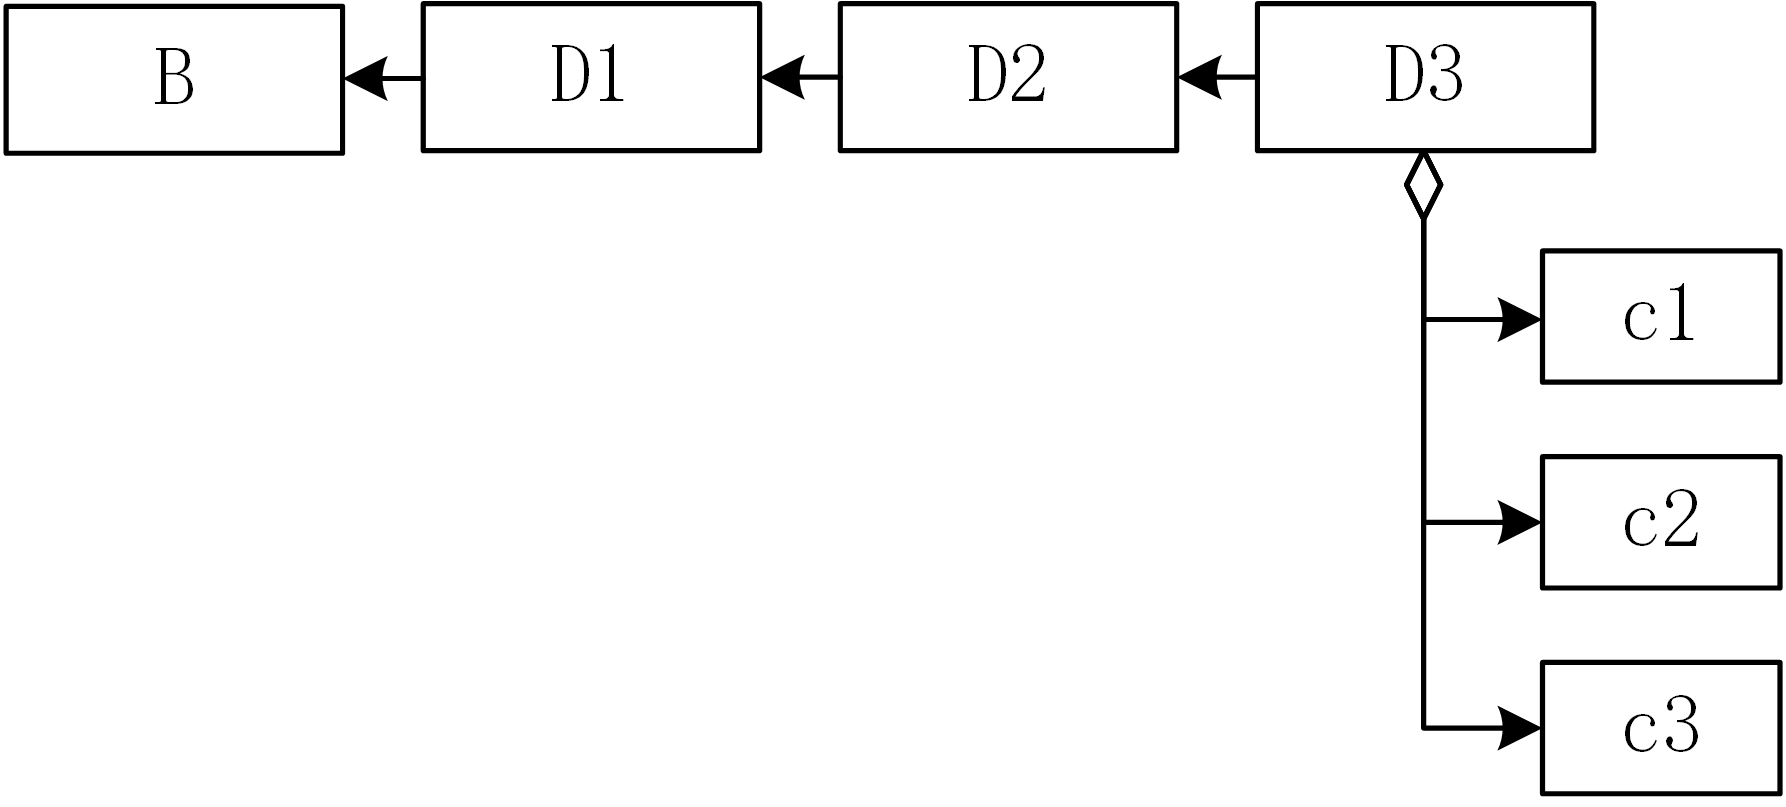
\includegraphics[width=0.8\textwidth]{Fig/Constr-Destr.png}
\end{figure}

构造顺序:\uncover<2->{B} \uncover<3->{D1} \uncover<4->{D2} \uncover<5->{D3}\uncover<6->{(c1} \uncover<7->{c2} \uncover<8->{c3)}

析构顺序:\uncover<9->{D3}\uncover<10->{(c3} \uncover<11->{c2} \uncover<12->{c1)} \uncover<13->{D2} \uncover<14->{D1} \uncover<15->{B}

\end{frame}
\subsection{派生类对象的构造}

\begin{frame}[fragile]
    {9.2 构造、拷贝控制与继承\small{—派生类对象的构造}}
    \begin{block}{派生类Student对象的构造}
        以上述Student类为例:
    \begin{columns}
    \begin{column}{0.06\linewidth}
    \end{column}
    \begin{column}{0.94\linewidth}
    \begin{lstlisting}[]
Student::Student(const string &name,int age,const Course &c):
    Person(name, age),/*初始化基类成员*/
    m_course(c)/*初始化自有成员*/ {
    cout<<"Constr of Student"<<endl;
}
    \end{lstlisting}\ttfamily
    \end{column}
    \end{columns}
        Student类中成员m\_course以复制构造的方式初始化。如下:
    \begin{columns}
    \begin{column}{0.06\linewidth}
    \end{column}
    \begin{column}{0.94\linewidth}
    \begin{lstlisting}[]
Course::Course(const Course &rhs): m_name(rhs.name),
    m_score(rhs.m_score) {
    cout<< "Copy constr of Course" <<endl;
}
    \end{lstlisting}\ttfamily
    \end{column}
    \end{columns}
    \end{block}
\end{frame}
\subsection{拷贝控制与继承}


\begin{frame}[fragile]
    {9.2 构造、拷贝控制与继承\small{—派生类对象的构造}}
    \begin{block}{派生类Student对象的构造}
        类似地,Person类初始化如下:
    \begin{columns}
    \begin{column}{0.06\linewidth}
    \end{column}
    \begin{column}{0.94\linewidth}
    \begin{lstlisting}[]
Person::Person(const string &name = "",int age = 0):
    m_name(name), m_age(age) {
    cout<<"Constr of Person"<<endl;
}
    \end{lstlisting}\ttfamily
    \end{column}
    \end{columns}
        当创建Student类对象时:\\\vspace{0.5em}
        Student s("Kevin", 19, Course("Math"));\\\vspace{0.5em}
        输出结果:\\\vspace{0.5em}
        Constr of Person\\
        Copy constr of Course\\
        Constr of Student\\
    \end{block}
    \begin{yellowblock}{提示:存在继承关系的类的成员初始化}
        在派生类对象构造过程中,每个类\alert{仅负责}自己的成员的初始化。
    \end{yellowblock}
\end{frame}

\begin{frame}[fragile]
    {9.2 构造、拷贝控制与继承\small{—拷贝控制与继承}}
    \begin{block}{析构与继承}
        类似于构造函数,Course、Student和Person类的析构函数的函数如下:
    \begin{columns}
    \begin{column}{0.06\linewidth}
    \end{column}
    \begin{column}{0.94\linewidth}
    \begin{lstlisting}[]
Person::~Person() {
    cout<< "Destr of Person" <<endl;
}
Student::~Student() {
    cout<< "Destr of Student" <<endl;
}
Course::~Course() {
    cout<< "Destr of Course" <<endl;
}
    \end{lstlisting}\ttfamily
    \end{column}
    \end{columns}
        利用如下代码创建Student类对象:\\\vspace{0.5em}
        Course c("Math");\\
        \{\\
          ~~~~Student s("Kevin", 19, c); ~~~~\texttt{//}\alert{思考}:输出结果会是怎样的? \\
        \}\\\vspace{0.5em}

    \end{block}
\end{frame}

\begin{frame}[fragile]
    {9.2 构造、拷贝控制与继承\small{—拷贝控制与继承}}
    \begin{block}{析构与继承}
        ~~输出结果:\\\vspace{0.5em}
        ~~Destr of Student\\
        ~~Destr of Course\\
        ~~Destr of Person\\
    \end{block}
\end{frame}

\begin{frame}[fragile]
    {9.2 构造、拷贝控制与继承\small{—拷贝控制与继承}}
    \begin{block}{复制、移动与继承}
        一个派生类对象在\alert{复制}或\alert{移动}的时候,除复制或移动自有成员外,还要复制或移动基类部分的成员。因此,通常在复制或移动构造函数的初始化列表中调用基类的\alert{复制或移动构造函数}。
    \begin{columns}
    \begin{column}{0.06\linewidth}
    \end{column}
    \begin{column}{0.94\linewidth}
    \begin{lstlisting}[]
class A{/*...*/};
class B : public A {
    string m_d;
public:
    B(const B &d):A(d) /* 复制A的成员 */,
        m_d(d.m_d) /* 复制B的成员 */ {
        /*...*/
    }
    B(B &&d):A(std::move(d)) /* 移动A的成员  */,
        m_d(std::move(d.m_d)) /* 移动B的成员  */ {
        /*...*/
    }
};
    \end{lstlisting}\ttfamily
    \end{column}
    \end{columns}
    \end{block}
\end{frame}

\begin{frame}[fragile]
    {9.2 构造、拷贝控制与继承\small{—拷贝控制与继承}}
    \begin{block}{赋值与继承}
        与复制和移动构造函数类似,必须在派生类的赋值运算符中\alert{显式}调用基类的赋值运算符,才能正确地完成基类成员的赋值:
    \begin{columns}
    \begin{column}{0.06\linewidth}
    \end{column}
    \begin{column}{0.94\linewidth}
    \begin{lstlisting}[]
B& B::operator=(const B &d) {
    if(this == &d) return *this;
    A::operator=(d);                  //赋值A的成员
    m_d = d.m_d;                      //赋值自身成员
    return *this;
}
    \end{lstlisting}\ttfamily
    \end{column}
    \end{columns}
    \end{block}
    \begin{yellowblock}{提示:派生类中使用基类的构造或赋值成员}
    ~~~~~~在派生类对象的构造或赋值过程中,无论基类相应的成员是编译器合成的还是自定义的,派生类都可以直接使用它们。如果基类中合成的构造函数、复制构造函数或赋值运算符是删除的或者是不可以访问的,那么派生类中对应的合成成员也是删除的,原因是派生类不能执行基类成员的构造、复制和赋值。
    \end{yellowblock}
\end{frame}

\section{虚函数与多态性}
\subsection{虚函数}

\begin{frame}[fragile]
    {9.3 虚函数与多态性\small{—虚函数}}
    \begin{block}{Shape、Circle和Square}
        下面定义了三个类:Shape、Circle和Square。
    \begin{columns}
    \begin{column}{0.06\linewidth}
    \end{column}
    \begin{column}{0.94\linewidth}
    \begin{lstlisting}[]
class Shape {
protected:
    string m_name;
public:
    Shape(const string &s = ""):m_name(s) { }
    virtual double area() const { return 0; }       //此函数为虚函数
    const string& name() { return m_name; }
};
class Circle : public Shape {
private:
    double m_rad;
public:
    Circle(double r=0, const string &s = ""):Shape(s),
        m_rad(r) { }
    double area() const { return 3.1415926*m_rad*m_rad; }
};
    \end{lstlisting}\ttfamily
    \end{column}
    \end{columns}
    \end{block}
\end{frame}

\begin{frame}[fragile]
    {9.3 虚函数与多态性\small{—虚函数}}
    \begin{block}{Shape、Circle和Square}
    \begin{columns}
    \begin{column}{0.06\linewidth}
    \end{column}
    \begin{column}{0.94\linewidth}
    \begin{lstlisting}[]
class Square : public Shape {
private:
    double m_len;
public:
    Square(double l=0, const string &s = ""):m_len(l) {}
    double area() const { return m_len*m_len; }
};
    \end{lstlisting}\ttfamily
    \end{column}
    \end{columns}
    \end{block}
\end{frame}

\subsection{动态绑定}

\begin{frame}[fragile]
    {9.3 虚函数与多态性\small{—动态绑定}}
    \begin{block}{静态类型和动态类型}
    \alert{静态类型}指对象声明时的类型或表达式生成时的类型,在编译时就已经确定,例如:
    \begin{columns}
    \begin{column}{0.06\linewidth}
    \end{column}
    \begin{column}{0.94\linewidth}
    \begin{lstlisting}[]
    class Base { }
    Base *p;        //指针p的静态类型为Base
    \end{lstlisting}\ttfamily
    \end{column}
    \end{columns}
    \alert{动态类型}指指针或引用所绑定的对象的类型,仅在运行时可知,例如:
    \begin{columns}
    \begin{column}{0.06\linewidth}
    \end{column}
    \begin{column}{0.94\linewidth}
    \begin{lstlisting}[]
    class Derived : public Base { };
    Derived d;
    Base *p = &d;   //指针p的动态类型为Derived
    \end{lstlisting}\ttfamily
    \end{column}
    \end{columns}
    \end{block}
\end{frame}

\begin{frame}[fragile]
    {9.3 虚函数与多态性\small{—动态绑定}}
    \begin{block}{动态绑定}
    ~~~~~~基类指针p的静态类型为Base,但它的动态类型为Derived。如果一个对象既不是指针也不是引用,那么它的静态类型和动态类型一致,比如d的静态类型和动态类型都是Derived。除需要重写基类的虚函数外,还必须用基类的指针或引用才能触发\alert{动态绑定},例如:
    \begin{columns}
    \begin{column}{0.06\linewidth}
    \end{column}
    \begin{column}{0.94\linewidth}
    \begin{lstlisting}[]
    Shape sh, *p = &sh;       //p指向Shape类对象
    Square sq(1.0);
    cout<<p->area()<<endl;    //打印输出0
    p = &sq;                  //将p绑定到sq
    cout<<p->area()<<endl;    //打印输出1.0
    \end{lstlisting}\ttfamily
    \end{column}
    \end{columns}
    \end{block}
\end{frame}

\begin{frame}[fragile]
    {9.3 虚函数与多态性\small{—动态绑定}}
    \begin{block}{动态绑定}
    ~~~~~~同样,可以利用基类的引用实现动态绑定,例如:
    \begin{columns}
    \begin{column}{0.06\linewidth}
    \end{column}
    \begin{column}{0.94\linewidth}
    \begin{lstlisting}[]
    bool operator>(const Shape &s1, const Shape &s2) {
        return s1.area()>s2.area();
    }
    Shape *p = nullptr;
    Square sq(2.0);
    Circle ci(1.2);
    if(sq>ci)         //调用重载的运算符>
        p = &sq;
    \end{lstlisting}\ttfamily
    \end{column}
    \end{columns}
    \end{block}
\end{frame}

\begin{frame}[fragile]
    {9.3 虚函数与多态性\small{—动态绑定}}
    \begin{block}{虚析构函数}
    ~~~~~~通常情况下,基类的析构函数应该是虚函数,保证正确delete一个动态派生类对象,例如:
    \begin{columns}
    \begin{column}{0.06\linewidth}
    \end{column}
    \begin{column}{0.94\linewidth}
    \begin{lstlisting}[]
    class Shape {
    public:
        virtual ~Shape() {
            cout<<"Destr of Shape"<<endl;
        }
    };
    class Circle : public Shape {
    public:
        ~Circle() {
            cout<<"Destr of Circle"<<endl;
        }
    };
    \end{lstlisting}\ttfamily
    \end{column}
    \end{columns}
    \end{block}
\end{frame}

\begin{frame}[fragile]
    {9.3 虚函数与多态性\small{—动态绑定}}
    \begin{block}{虚析构函数}
    ~~~~~~运行如下代码:
    \begin{columns}
    \begin{column}{0.06\linewidth}
    \end{column}
    \begin{column}{0.94\linewidth}
    \begin{lstlisting}[]
    Shape *p = new Circle();
    delete p;
    \end{lstlisting}\ttfamily
    \end{column}
    \end{columns}
    ~~~~~~由于Shape类的析构函数为\alert{虚函数},因此在执行delete操作时,将会执行p的动态类型的析构函数,即派生类Circle的析构函数,然后再执行基类Shape的析构函数,从而保证p指向的动态Circle类对象能够\alert{正确释放内存}。上面代码执行delete操作将输出:\\\vspace{0.5em}
    ~~~~~~Destr of Circle\\
    ~~~~~~Destr of Shape\\\vspace{0.5em}
    ~~~~~~如果基类析构函数为非虚函数,则delete一个指向派生类对象的基类指针将产生\alert{未定义的行为}。
    \end{block}
\end{frame}

\begin{frame}[fragile]
    {9.3 虚函数与多态性\small{—动态绑定}}
    \begin{yellowblock}{提示:虚析构函数将阻止移动运算的合成}
    ~~~~~~基类中的虚析构函数将阻止编译器合成移动操作,通过\texttt{=}default形式使用合成的析构函数也会产生同样的影响。
    \end{yellowblock}
    \begin{block}<2->{注意}
    ~~~在使用虚函数时:
    \begin{itemize}[<+(2)->]
    \item 动态绑定必须通过基类\alert{指针}或\alert{引用}绑定到派生类对象才能触发。
    \item 若基类的某个函数被声明为虚函数,则派生类中对应的重写版本\alert{自动}为虚函数,可不必进行virtual声明。
    \item 内联成员、静态成员和模板成员均不能声明为虚函数,因为这些成员的行为必须在编译时确定,不能实现动态绑定。
    \item 动态绑定的实现是有\alert{代价}的。每个派生类需要额外的空间保存虚函数的入口地址,函数的调用机制也是间接实现的,动态绑定的实现是以时间和空间为代价的,因此大量的虚函数会导致程序性能的下降。
    \item 派生类版本的声明必须与基类版本的声明完全一致,包括函数名、形参列表和返回值类型。
    \end{itemize}
    \end{block}
\end{frame}

\begin{frame}[fragile]
    {9.3 虚函数与多态性\small{—动态绑定}}

\begin{columns}[t]
\column{0.65\textwidth}
    \begin{block}{}
    \vspace{-3mm}\begin{lstlisting}[moreemph={Base,Derived}]
class Base {
public:
    virtual Base* foo() { cout << "Base" << endl; return this; }
};
class Derived : public Base {
public:
    Derived* foo() { cout << "Derived" << endl; return this; }
};
void test() {
    Derived d;
    Base *p = &d;
    p->foo();
    d.foo();
}
    \end{lstlisting}\vspace{-3mm}
    \end{block}
\column{0.3\textwidth}
    \begin{block}{例外}
    基类版本返回基类指针或引用,派生类版本可以返回派生类指针或引用
    \end{block}
    \end{columns}

\vspace{2mm}

调用\texttt{test()}函数输出:\\
\texttt{Derived}\\\texttt{Derived}

\end{frame}

\begin{frame}[fragile]
    {9.3 虚函数与多态性\small{—动态绑定}}

\begin{columns}[t]
\column{0.65\textwidth}
    \begin{block}{}
    \vspace{-3mm}\begin{lstlisting}[moreemph={Base,Derived}]
class Base{
public:
    virtual void fun(int i=0) {
        cout << "Base:" << i << endl; }
};
class Derived : public Base{
public:
    void fun(int i=1) {
        cout << "Derived:" << i << endl; }
};
void test(){
    Derived d;
    Base *p = &d;
    p->fun();
    d.fun();
}
    \end{lstlisting}\vspace{-3mm}
    \end{block}
    \column{0.3\textwidth}
    \begin{block}{注意}
    如果参数具有默认值,则各个版本中对应形参的\alert{默认值必须相同}\\
    \end{block}

    \end{columns}

    \vspace{2mm}

调用\texttt{test()}函数输出:\\
\texttt{Derived:0}\\\texttt{Derived:1}
\end{frame}

\begin{frame}[fragile]
    {9.3 虚函数与多态性\small{—动态绑定}}
    \begin{block}{final和override说明符}
    ~~~~~~C++11~引入了关键字~override\index{O!override}~用来\alert{显式}说明派生类的函数要覆盖基类的虚函数。类似的,可以使用关键字~final\index{F!final}~\alert{阻止}派生类覆盖基类版本的虚函数。
    \begin{columns}
    \begin{column}{0.06\linewidth}
    \end{column}
    \begin{column}{0.94\linewidth}
    \begin{lstlisting}[]
struct B {
    virtual void fun1(int) { }
    virtual void fun2() { }
    void fun3() { }
};
struct D1 : public B {
    void fun1() override { }   //错误:基类没有不带参数的fun1函数
    void fun2() final { }        //D1::fun2为最终版本
    void fun3() override { }   //错误:基类没有可覆盖的函数
};
struct D2 : public D1 {
    void fun2() { }            //错误:不允许覆盖基类D1中的fun2函数
};
    \end{lstlisting}\ttfamily
    \end{column}
    \end{columns}
    \end{block}
\end{frame}
\subsection{抽象类}

\begin{frame}[fragile]
    {9.3 虚函数与多态性\small{—抽象类}}
    \begin{block}{纯虚函数}
    ~~~~~~上面定义的~Shape~类,实际上并不代表具体的几何形状类,因此它的成员函数~area~的定义是没有意义的,Shape~类只是几何形状的一个抽象,因此也不希望用户创建一个~Shape~类对象。C++~允许将这样的虚函数声明为\alert{纯虚}(pure virtual\index{P!pure virtual})函数:
    \begin{columns}
    \begin{column}{0.06\linewidth}
    \end{column}
    \begin{column}{0.94\linewidth}
    \begin{lstlisting}[]
    class Shape {
    public:
        virtual double area() const = 0;      //纯虚函数
        /*...*/
    }
    Shape sh;                //错误:不能创建抽象类的实例
    \end{lstlisting}\ttfamily
    \end{column}
    \end{columns}
    \end{block}
\end{frame}

\begin{frame}[fragile]
    {9.3 虚函数与多态性\small{—抽象类}}
    \begin{yellowblock}{提示:公有继承方式下的基类成员函数的继承与覆盖}
    \begin{itemize}
    \item 不要重新定义基类非虚函数,所有作用于基类的非虚操作都适用于它的派生类。
    \item 如果需要重新定义基类函数,则该函数应声明为虚函数。
    \item 派生类继承基类非虚函数的接口和实现、虚函数的接口和默认实现,以及纯虚
函数的接口。
    \end{itemize}
    ~~~~~~一般情况下,对纯虚函数不需要定义,但可以为纯虚函数提供定义,而且必须放在
类外。
    \end{yellowblock}
\end{frame}
\subsection{继承与组合}

\begin{frame}[fragile]
    {9.3 虚函数与多态性\small{—继承与组合}}
    \begin{block}{Cat和Dog}
    \begin{columns}
    \begin{column}{0.06\linewidth}
    \end{column}
    \begin{column}{0.94\linewidth}
    \begin{lstlisting}[]
    class Cat {
    protected:
        string m_name;
    public:
        void meow() {     //喵喵叫
            cout<<"meowing"<<endl;
        }
    };
    class Dog {
    protected:
        string m_name;
    public:
        void bark() {     //汪汪叫
            cout<<"barking"<<endl;
        }
    };
    \end{lstlisting}\ttfamily
    \end{column}
    \end{columns}
    \end{block}
\end{frame}

\begin{frame}[fragile]
    {9.3 虚函数与多态性\small{—继承与组合}}
    \begin{block}{IS-A设计}
    ~~~~~~改写Dog类如下:
    \begin{columns}
    \begin{column}{0.06\linewidth}
    \end{column}
    \begin{column}{0.94\linewidth}
    \begin{lstlisting}[]
    class Dog : public Cat {
    public:
        void bark();
    };
    Dog dog;          //创建一个Dog类对象
    dog.bark();       //调用bark函数
    \end{lstlisting}\ttfamily
    \end{column}
    \end{columns}
    ~~~~~~虽然dog能汪汪叫,但是它也会喵喵叫,因为Dog类继承了Cat类的meow函数,显然这是\alert{不符合}事实的,Dog不是一种Cat,显然不是\alert{属于}关系。
    \end{block}
\end{frame}

\begin{frame}[fragile]
    {9.3 虚函数与多态性\small{—继承与组合}}
    \begin{block}{HAS-A设计}
    ~~~~~~改写Dog类如下:
    \begin{columns}
    \begin{column}{0.06\linewidth}
    \end{column}
    \begin{column}{0.94\linewidth}
    \begin{lstlisting}[]
    class Dog {
        Cat m_cat;
    public:
        void bark();
    };
    \end{lstlisting}\ttfamily
    \end{column}
    \end{columns}
    ~~~~~~在这种设计中,虽然dog不能喵喵叫了(不能直接调用meow函数),但这种设计\alert{不符合}自然逻辑,Dog和Cat类显然不是\alert{组合}关系。
    \end{block}
\end{frame}

\begin{frame}[fragile]
    {9.3 虚函数与多态性\small{—继承与组合}}
    \begin{block}{抽象共有属性设计}
    ~~~~~~把Cat和Dog共有的属性\alert{抽象}出来,包括名字和发声行为,从而形成一个新的公共基类Mammal:
    \begin{columns}
    \begin{column}{0.06\linewidth}
    \end{column}
    \begin{column}{0.94\linewidth}
    \begin{lstlisting}[]
    class Mammal {
    protected:
        string m_name;
    public:
        virtual void sounding() = 0;
    };
    class Cat : public Mammal {
    protected:
        void meow();
    public:
        void sounding() override { meow(); }
    };
    \end{lstlisting}\ttfamily
    \end{column}
    \end{columns}
    \end{block}
\end{frame}

\begin{frame}[fragile]
    {9.3 虚函数与多态性\small{—继承与组合}}
    \begin{block}{抽象共有属性设计}
    \begin{columns}
    \begin{column}{0.06\linewidth}
    \end{column}
    \begin{column}{0.94\linewidth}
    \begin{lstlisting}[]
    class Dog : public Mammal {
    protected:
        void bark();
    public:
        void sounding() override { bark(); }
    };
    \end{lstlisting}\ttfamily
    \end{column}
    \end{columns}
    ~~~~~~在上面的设计中,既统一了接口,又实现了不同的行为。这种设计也\alert{符合}事实和自然逻辑。下面的dog和cat也有了正常的行为:\\\vspace{0.5em}
    ~~~~~~Dog dog; Cat cat;\\
    ~~~~~~dog.sounding();  ~~~~~~\texttt{//}dog能正常的汪汪叫\\
    ~~~~~~cat.sounding();  ~~~~~~\texttt{//}cat能正常的喵喵叫\\
    \end{block}
\end{frame}
\subsection{再探计算器}
\begin{frame}[fragile]
    {9.3 虚函数与多态性\small{—再探计算器}}
    \begin{thinkblock}{思考:}
    ~~~~~~在前面章节,利用链栈实现了一个简单的计算器程序。经过学习本章节后,如何利用OOP思想重新设计与实现计算机程序?
    \end{thinkblock}\vspace{4em}
    %\begin{beamercolorbox}[rounded=true, shadow=false,wd=0pt]{bgcolor}
    
\includegraphics[scale=0.6]{Fig/question_fig.jpg}
    %\end{beamercolorbox}
\end{frame}

\begin{frame}[fragile]
    {9.3 虚函数与多态性\small{—再探计算器}}
    \begin{block}{定义运算符基类}
    ~~~~~~把每一种运算符抽象成一个类,再把运算符的\alert{共有属性抽象}出来,形成一个公共基类Operator。运算符继承关系如下:
    \end{block}\vspace{2em}
    \begin{figure}
    \centering
    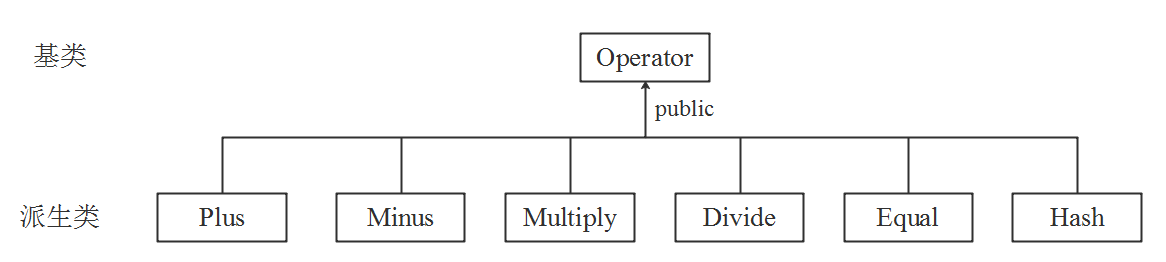
\includegraphics[width=30em]{Fig/Operator.png}
    \end{figure}
\end{frame}

\begin{frame}[fragile]
    {9.3 虚函数与多态性\small{—再探计算器}}
    \begin{block}{定义运算符基类}
    ~~~~~~基类Operator和它的派生类如下:
    \begin{columns}
    \begin{column}{0.06\linewidth}
    \end{column}
    \begin{column}{0.94\linewidth}
    \begin{lstlisting}[]
class Operator{
public:
    Operator(char c, int numOprd, int pre) :
        m_symbol(c), m_numOprand(numOprd), m_precedence(pre){}
    char symbol() const { return m_symbol; }
    int numOprand() const { return m_numOprand; }
    int precedence() const { return m_precedence; };
    virtual double get(double a, double b) const = 0;
    virtual ~Operator() {}
protected:
    const char m_symbol;      //符号
    const int m_numOprand;    //目数
    const int m_precedence;   //优先级
};
    \end{lstlisting}\ttfamily
    \end{column}
    \end{columns}
    \end{block}
\end{frame}

\begin{frame}[fragile]
    {9.3 虚函数与多态性\small{—再探计算器}}
    \begin{block}{定义运算符基类}
    \begin{columns}
    \begin{column}{0.06\linewidth}
    \end{column}
    \begin{column}{0.94\linewidth}
    \begin{lstlisting}[]
class Plus : public Operator{     //运算符 +
public:
    Plus() :Operator('+', 2, 2) {}
    double get(double a, double b) const { return a + b; }
};
class Minus :public Operator{     //运算符 -
public:
    Minus() :Operator('-', 2, 2) {}
    double get(double a, double b) const { return a - b; }
};
class Multiply :public Operator{  //运算符 *
public:
    Multiply() :Operator('*', 2, 3) {}
    double get(double a, double b) const { return a * b; }
};
    \end{lstlisting}\ttfamily
    \end{column}
    \end{columns}
    \end{block}
\end{frame}

\begin{frame}[fragile]
    {9.3 虚函数与多态性\small{—再探计算器}}
    \begin{block}{定义运算符基类}
    \begin{columns}
    \begin{column}{0.06\linewidth}
    \end{column}
    \begin{column}{0.94\linewidth}
    \begin{lstlisting}[]
class Divide :public Operator{      //运算符 /
public:
    Divide() :Operator('/', 2, 3) {}
    double get(double a, double b) const { return a / b; }
};
class Hash :public Operator{        //运算符 #
public:
    Hash() :Operator('#', 1, 1) {}  //函数get无实际意义,仅为语                                              法正确
    double get(double a, double b) const { return a; }
};
class Equal :public Operator{       //表达介绍符  =
public:
    Equal() :Operator('=', 2, 0) {} //函数get无实际意义,仅为语                                              法正确
    double get(double a, double b) const { return a; }
};
    \end{lstlisting}\ttfamily
    \end{column}
    \end{columns}
    \end{block}
\end{frame}

\begin{frame}[fragile]
    {9.3 虚函数与多态性\small{—再探计算器}}
    \begin{block}{定义计算器类}
    ~~~~~~由于unique\_ptr不支持复制操作,因此向前面章节定义的Node模板和Stack模板分别添加支持移动语义的构造函数和push函数:
        \begin{lstlisting}[basicstyle=\normalsize\ttfamily]
        template<typename T>    // 含右值形参的移动构造函数
        Node<T>::Node(T &&val) :m_value(std::move(val)) { }
        template<typename T>
        void Stack<T>::push(T &&val) {  //含右值形参的push函数
            Node<T> *node = new Node<T>(std::move(val));
            node->m_next = m_top;
            m_top = node;
        }
\end{lstlisting}
    \end{block}
\end{frame}

\begin{frame}[fragile]
    {9.3 虚函数与多态性\small{—再探计算器}}
    \begin{block}{定义计算器类}
    ~~~~~~Calculator类的定义如下:
    \begin{columns}
    \begin{column}{0.06\linewidth}
    \end{column}
    \begin{column}{0.94\linewidth}
    \begin{lstlisting}[]
class Calculator {
private:
    Stack<double> m_num;               //操作数栈
    Stack<unique_ptr<Operator>> m_opr; //运算符数栈
    void calculate();
    //成员函数readNum和isNum与前面章节定义的相同
public:
    Calculator(){ m_opr.push(make_unique<Hash>()); } //调用移动push函数
    double doIt(const string &exp);
};
    \end{lstlisting}\ttfamily
    \end{column}
    \end{columns}
    \end{block}
\end{frame}

\begin{frame}[fragile]
    {9.3 虚函数与多态性\small{—再探计算器}}
    \begin{block}{定义计算器类}
    \begin{columns}
    \begin{column}{0.06\linewidth}
    \end{column}
    \begin{column}{0.94\linewidth}
    \begin{lstlisting}[]
void Calculator::calculate(){   //操作数出栈并进行相应计算
    double a[2] = {0};
    for (auto i = 0; i < m_opr.top()->numOprand(); ++i) {
        a[i] = m_num.top();
        m_num.pop();
    }//调用绑定的函数对象进行表达式运算,并将计算结果压栈
    m_num.push(m_opr.top()->get(a[1],a[0]));//注意操作数的顺序
    m_opr.pop();
}
    \end{lstlisting}\ttfamily
    \end{column}
    \end{columns}
    \end{block}
\end{frame}

\begin{frame}[fragile]
    {9.3 虚函数与多态性\small{—再探计算器}}
    \begin{block}{定义计算器类}
    \begin{columns}
    \begin{column}{0.06\linewidth}
    \end{column}
    \begin{column}{0.94\linewidth}
    \begin{lstlisting}[]
double Calculator::doIt(const string & exp){
    for (auto it = exp.begin(); it != exp.end();){
        if (isNum(it))  //如果是操作数, 则将其压栈
            m_num.push(readNum(it));
        else{   //根据当前运算符创建相应的派生类对象
            char o = *it++;
            unique_ptr<Operator> oo; //定义基类指针
            if (o == '+')
                oo = make_unique<Plus>();//与Plus对象绑定,触发移动语义
            else if (o == '-')
                oo = make_unique<Minus>();//与Minus对象绑定
            else if (o == '*')
                oo = make_unique<Multiply>();//与Multiply绑定
            else if (o == '/')
                oo = make_unique<Divide>();//与Divide对象绑定
    \end{lstlisting}\ttfamily
    \end{column}
    \end{columns}
    \end{block}
\end{frame}

\begin{frame}[fragile]
    {9.3 虚函数与多态性\small{—再探计算器}}
    \begin{block}{定义计算器类}
    \begin{columns}
    \begin{column}{0.06\linewidth}
    \end{column}
    \begin{column}{0.94\linewidth}
    \begin{lstlisting}[]
            else if (o == '=')
                oo = make_unique<Equal>();//与Equal对象绑定
            while (oo->precedence()<=m_opr.top()->precedence()){
                if (m_opr.top()->symbol() == '#')
                    break;
                calculate(); //根据栈顶运算符,执行相应计算
            }
            if( oo->symbol() != '=')//除=以外,其它运算符入栈
                m_opr.push(std::move(oo));//将oo转换为右值,调用移动push函数
        }
    }
    double result = m_num.top();
    m_num.pop();
    return result;
}
    \end{lstlisting}\ttfamily
    \end{column}
    \end{columns}
    \end{block}
\end{frame}

\begin{frame}[fragile]
    \frametitle{~~}
    \begin{center}
\huge{本章结束}
\end{center}
\end{frame}

\end{document} 